\documentclass[10pt]{article}
\pdfoutput=1
%\usepackage{NotesTeX,lipsum}
\usepackage{NotesTeX,lipsum}
%\usepackage{showframe}

\title{\begin{center}{\Huge \textit{Notes}}\\{{\itshape Research}}\end{center}}
\author{Yi Huang}


\affiliation{
University of Minnesota
}

\emailAdd{huan1756@umn.edu}

\begin{document}
	\maketitle
	\flushbottom
	\newpage
	\pagestyle{fancynotes}
	\part{Spring 2019}
	\section{Capacitor}\label{sec:capacitor}
	\begin{margintable}\vspace{.8in}\footnotesize
		\begin{tabularx}{\marginparwidth}{|X}
		Section~\ref{sec:capacitor}. Spring 2019\\
		\end{tabularx}
	\end{margintable}

	\graphicspath{ {./images/} }

\subsection{Energy of one-dimensional Capacitor}

If dipoles are aligned along the diameter of the circle, i.e. there are only parallel or antiparallel dipoles in the one-dimensional capacitor, we can compute the electrostatic energy as follows:

\begin{equation}
	E = \frac{1}{2} nL (U_e + U_h) + nL eV_1,
\end{equation}
where $n$ is the electron density ($a=1/n$ is the lattice constant), $L$ is the length of the cylinder, $U_e$ is the interaction energy per electron along the center axis of the cylinder, $U_h$ is the interaction energy per hole in the cylinder surface, and $V_1$ is the voltage to create a single dipole.

For the electron at the origin
\begin{equation}
	U_e = \frac{e^2}{\epsilon} \sum_{\alpha \neq 0} \qty(\frac{1}{r_{\alpha}} - \frac{1}{\sqrt{r_{\alpha}^2 + R^2}})
\end{equation}
where $R$ is the radius of the cylinder, $\alpha$ is an index labelling the position of the electrons in the center axis, and $\alpha \neq 0$ denotes we sum over all positon except the origin.
\begin{align*}
	U_e &= \frac{e^2}{\epsilon} \sum_{i \neq 0} \qty(\frac{1}{ia} - \frac{1}{\sqrt{(ia)^2 + R^2}}) \\
	&= \frac{ne^2}{\epsilon} 2\sum_{i=1}^{\infty} \qty(\frac{1}{i} - \frac{1}{\sqrt{i^2 + (nR)^2}}) \\
	&= \frac{ne^2}{\epsilon} g(nR).
\end{align*}
where
\begin{equation}
	g(x) = 2\sum_{i=1}^{\infty} \qty(\frac{1}{i} - \frac{1}{\sqrt{i^2 + x^2}}),
\end{equation}
if $x\ll 1$, we can expand $g(x)$ in powers of $x^2$
\begin{align*}
	g(x) &= 2\sum_{i=1}^{\infty} \frac{1}{i}\qty(1 - \frac{1}{\sqrt{1 + (x/i)^2}}) \\
	&= 2\sum_{i=1}^{\infty} \frac{1}{i}\qty(1 - 1 + \frac{1}{2} \frac{x^2}{i^2} + O(x^4))\\
	&= x^2 \sum_{i=1}^{\infty} \frac{1}{i^3} + O(x^4)\\
	&= \zeta(3) x^2 + O(x^4) \approx 1.20 x^2.
\end{align*}

For the hole at the origin we can divide the energy into two parts $U_h = U_{h1} + U_{h2}$. The contribution from the interaction of hole with the same orientation as the origin dipole is
\begin{align*}
	U_{h1} &= \frac{e^2}{\epsilon} \sum_{\alpha \neq 0}{}^{'} \qty(\frac{1}{r_{\alpha}} - \frac{1}{\sqrt{r_{\alpha}^2 + R^2}})\\
	&= \frac{ne^2}{2\epsilon} g(nR/2),
\end{align*}
while the contribution from the antiparallel dipole is
\begin{align*}
	U_{h2} &= \frac{e^2}{\epsilon} \sum_{\alpha \neq 0}{}^{''} \qty(\frac{1}{\sqrt{r_{\alpha}^2 + 4R^2}} - \frac{1}{\sqrt{r_{\alpha}^2 + R^2}}) \\
	&= \frac{ne^2}{\epsilon} h(nR),
\end{align*}
where
\begin{equation}
	h(x) = 2\sum_{i=0}^{\infty} \qty(\frac{1}{\sqrt{(2i+1)^2 + 4x^2}} - \frac{1}{\sqrt{(2i+1)^2 + x^2}}).
\end{equation}
If $x \ll 1$, we can expand $h(x)$
\begin{align*}
	h(x) &= -3x^2 \sum_{i=0}^{\infty} \frac{1}{(2i+1)^3} + O(x^4) \\
	&= -\frac{21 \zeta(3)}{8} x^2 +O(x^4) \approx -3.15x^2.
\end{align*}

If dipoles are not aligned, for example, they are separated by an angle instead of $\pi$ but $2\pi/3$, we can calculate its energy similarly.

Obviously, the interaction energy from the electrons in the center line doesn't change, so we only need to calculate the interaction energy from the holes. The parallel dipole contribution is
\begin{equation}
	U_{h1} = \frac{ne^2}{3\epsilon} g(nR/3),
\end{equation}
while the nonparallel dipole contribution is
\begin{align*}
	U_{h_2} &= \frac{e^2}{\epsilon} \sum_{\alpha \neq 0}{}^{'''} \qty(\frac{1}{\sqrt{r_{\alpha}^2 + 3R^2}} - \frac{1}{\sqrt{r_{\alpha}^2 + R^2}}) \\
	&= \frac{ne^2}{\epsilon} f(nR),
\end{align*}
where
\begin{align*}
	f(x) =& 2\sum_{i=0}^{\infty} \left(\frac{1}{\sqrt{(3i+1)^2 + 3x^2}} + \frac{1}{\sqrt{(3i+2)^2 + 3x^2}} \right.\\
	& \left.- \frac{1}{\sqrt{(3i+1)^2 + x^2}} - \frac{1}{\sqrt{(3i+2)^2 + x^2}} \right).
\end{align*}
If $x \ll 1$, we can expand $f(x)$
\begin{align*}
	f(x) &= -2x^2\sum_{i=0}^{\infty} \qty(\frac{1}{(3i+1)^3} + \frac{1}{(3i+2)^3}) +O(x^4)\\
	&=-\frac{52\zeta(3)}{27} x^2 + O(x^4) \approx -2.32x^2.
\end{align*}
The picture of $g(x)$, $h(x)$, and $f(x)$ are shown in Fig. \ref{fig: 1}.

\begin{figure}[H]
	\centering
	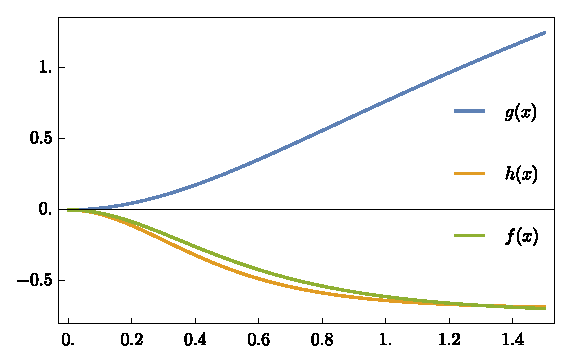
\includegraphics[height=7cm]{functions.eps}
	\caption{(Color online.) The picture of $g(x)$, $h(x)$, and $f(x)$.}
	\label{fig: 1}
\end{figure}

As a first glance, we can compare $U_h$ in the two different configurations in the limit $nR \ll 1$. If the dipoles are aligned, $U_h \approx -3 (nR)^2$; if the dipoles are separated by $2\pi/3$, $U_h \approx -2.27 (nR)^2$. This is as expected, because when the density is low, the interaction energy will be dominated by the nearest neighbor interaction, holes will be closer to its nearest neighbor if the dipoles are not aligned, and thus increase the repulsion. However, if $nR \gg 1$, holes will be closer to each other in the aligned case than the spread out case. Therefore we expect a transition $(nR)_1$ where the two configurations have the same energy. This is exactly what happens in the numerical result (see Fig. \ref{fig: 2}), with $(nR)_1 = 0.747$.

\begin{figure}[H]
	\centering
	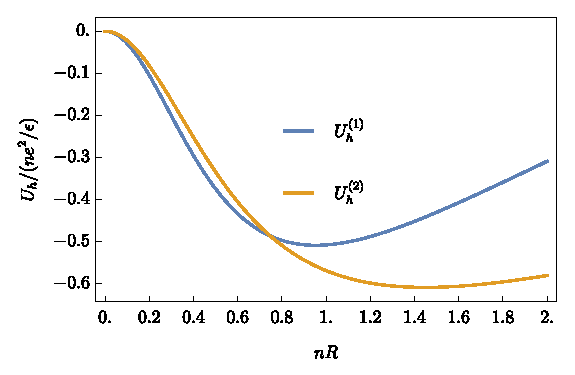
\includegraphics[height=7cm]{hole_energy.eps}
	\caption{(Color online.) The blue line $U_h^{(1)}$ shows the interaction energy from holes in the case that dipoles align in the diameter, while the yellow line $U_h^{(2)}$ shows the interaction energy from holes where nearest neighbor dipole spread out by angle $2\pi/3$.}
	\label{fig: 2}
\end{figure}

We can write $U \equiv E - enLV_1$ as
\begin{equation}
	U = \frac{e^2n^2L}{2\epsilon} \qty(g(nR) + \frac{1}{2} g(nR/2) + h(nR)).
\end{equation}



\subsection{Density as a function of voltage $n(V)$}

The voltage can be related to energy as $V = \dv*{E}{q}$, where $\dd{q} = eL \dd{n}$, so we have
\begin{equation}
	V = V_1 + \frac{1}{eL} \dv{U}{n},
\end{equation}
or explicitly
\begin{align*}
	V-V_1 =& \frac{e}{\epsilon R} \frac{(nR)^2}{2} \qty(g'(nR) + \frac{1}{4} g'(nR/2) + h'(nR)) \\
	&+ \frac{e}{\epsilon R} nR \qty(g(nR) + \frac{1}{2} g(nR/2) + h(nR)).
\end{align*}

In principle, we can reverse the function $V(n)$ to get $n(V)$, but here $n(V)$ is actually multi-valued, which implies a first order phase transition.

\begin{figure}[H]
	\centering
	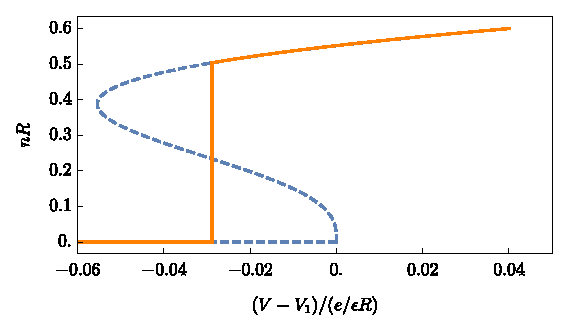
\includegraphics[height=7cm]{phase_transition.eps}
	\caption{(Color online.) The dimensionless density $nR$ as a function of dimensionless voltage $(V-V_1)/(e/\epsilon R)$ for the one-dimensional capacitor. The dashed curve shows the curve $n(V)$, while the orange curve shows a first order phase transition obtained using Maxwell's equal-area rule. We see that in equilibrium, the density jumps to a value $n_c R = 0.504$ at the criticla voltage $(V_c-V_1)/(e/\epsilon R) = -0.029$.}
	\label{fig: 3}
\end{figure}

\subsection{Capacitance}

First we discuss the geometric capacitance of a cylindrical capacitance. Use Gauss's law, we have the electric field inside the cylinder
\begin{equation}
	E = \frac{2en}{\epsilon \rho},
\end{equation}

Assume the inner line has a finite radius $b$, and $b \ll R$, then the voltage difference is
\begin{equation}
	V = \frac{2en}{\epsilon} \int_b^R \dd{\rho} \frac{1}{\rho} = \frac{2en}{\epsilon} \ln(\frac{R}{b}).
\end{equation}
Thus the geometric capacitance is
\begin{equation}
	C_g = \frac{Q}{V} = \frac{\epsilon L}{2 \ln(\frac{R}{b})}.
\end{equation}

Next we consider the differential capacitance of our one-dimensional device
\begin{equation}
	C^{-1} = \dv{V}{Q} = \dv[2]{E}{Q} = \frac{1}{(eL)^2} \dv[2]{E}{n}.
\end{equation}
Using $U = \frac{2 e^2 L}{\epsilon R^2} u(nR)$ where
\begin{equation}
	u(x) = \frac{x^2}{4} \qty(g(x) + \frac{1}{2} g(x/2) + h(x)),
\end{equation}
so explicitly, we have
\begin{equation}
	C^{-1} = \frac{2}{\epsilon L} u''(nR).
\end{equation}

Since the density $n(V)$ is a function of voltage, we can express our capacitance as a function of voltage
\begin{equation}
	C(V) = C_u(V) + en_cL \delta(V-V_c)
\end{equation}
where the non-singular capacitance $C_u(V)$ is obtained by differentiating the upper branch of the $n(V)$ curve.
\begin{figure}[H]
	\centering
	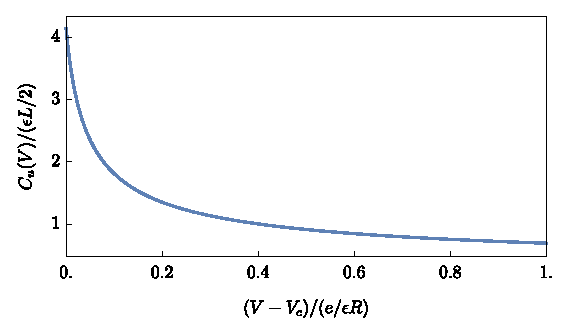
\includegraphics[height=7cm]{capacitance.eps}
	\caption{(Color online.) The dimensionless capacitance $C_u(V)/(\epsilon L/2)$ as a function of dimensionless voltage $(V-V_c)/(e/\epsilon R)$. Notice that because of the divergent nature of the line charge, we have an extra amplification factor $\ln(R/b)$ in the geometric capacitance $C_u(V)/C_g = \ln(R/b) C_u(V)/(\epsilon L/2)$. Thus this plot basically show us the case when $R/b = \e$. If $R/b = 10$, then $C_u/C_g$ is about 10.}
	\label{fig: 4}
\end{figure}

By varying the ratio $R/b$, we can obtain the critical ratio radius of the cylinder $(R/b)_0$ such that $C_u = C_g$, i.e.
\begin{equation}
	\qty(\frac{R}{b})_0 = \exp(\frac{\epsilon L}{2 C_u(V)})
\end{equation}
which is a function of $V$, and if $R/b > (R/b)_0$, $C_u > C_g$, otherwise $C_u < C_g$. See Figure \ref{fig: 5}.

\begin{figure}[H]
	\centering
	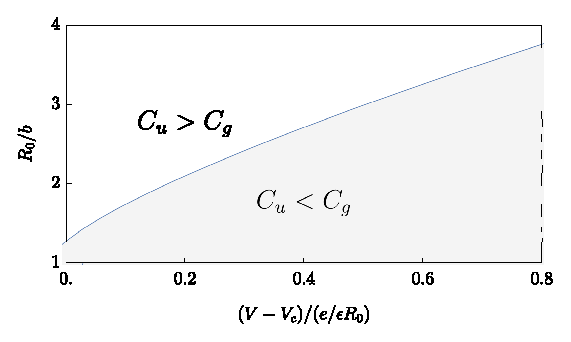
\includegraphics[height=7cm]{ratio_radius.eps}
	\caption{(Color online.) The critical ratio radius $(R/b)_0$ as a function of dimensionless voltage $(V-V_c)/(e/\epsilon R)$.}
	\label{fig: 5}
\end{figure}






\end{document}
